% ================================================================ results (v3)
% Generated numbers: v3/build_v3.py (\V{r3_*}); Methods numbers: build.py. Lines marked % [Cn] state a direction that
% v3/CLAIMS.md checks against the data; a failing claim means the sentence must be rewritten, not the number.
\section{Results}

\V{r3_banner}

\subsection{Primary comparison}\label{sec:res_primary}

\begin{figure}[!t]
  \centering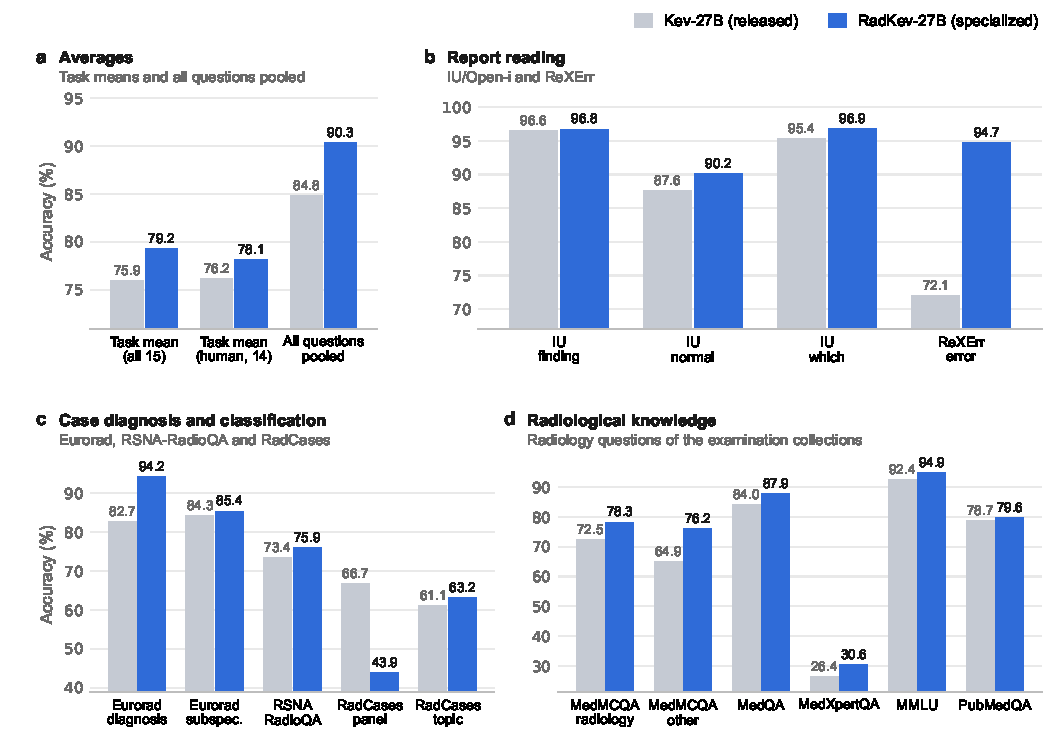
\includegraphics[width=\textwidth]{figures/v3_fig_primary.pdf}
  \caption{Accuracy of Kev-27B (grey) and of RadKev-27B (blue), the model specialized from it, on the radiology benchmark. (a) Averages: the unweighted mean of the task accuracies over all \V{r3_ntask} tasks (the primary outcome) and over the \V{r3_nhtask} tasks with human-assigned keys, and accuracy over all \V{r3_nq} questions. (b) Report reading: IU/Open-i (finding present, normal study, which finding) and ReXErr (whether a report contains an error; keys known by construction). (c) Case diagnosis and classification: Eurorad diagnosis and subspecialty, RSNA-RadioQA, and the ACR Appropriateness Criteria panel and topic of RadCases. (d) Radiological knowledge: the radiology questions of the examination collections. Differences and 95\% confidence intervals are given in the text and in Supplementary Table~\ref{tab:v3_primary_tasks}. Each accuracy axis spans 5 percentage points below the lowest and above the highest value in its panel.}
  \label{fig:primary}
\end{figure}

Averaged over the \V{r3_ntask} benchmark tasks, the prespecified primary outcome, accuracy was \V{r3_a_v3_27_tm}\% for RadKev-27B and \V{r3_a_stock27_tm}\% for Kev-27B, a difference of \V{r3_prim_tm} percentage points (95\% CI \V{r3_prim_tm_ci}; Figure~\ref{fig:primary}a). % [C1]
Over the \V{r3_nhtask} tasks with human-assigned keys, the difference was \V{r3_prim_htm} points (\V{r3_prim_htm_ci}), and over all \V{r3_nq} benchmark questions, each weighted equally, \V{r3_prim_pool} points (\V{r3_prim_pool_ci}). % [C2]
The per-task differences ranged from \V{r3_prim_tmin} points (\V{r3_prim_tmin_task}) to \V{r3_prim_tmax} points (\V{r3_prim_tmax_task}), and after Holm adjustment across the \V{r3_ntask} tasks (Supplementary Table~\ref{tab:v3_primary_tasks}), RadKev-27B was \V{r3_prim_holm}.

In report reading (Figure~\ref{fig:primary}b), the difference was \V{r3_prim_t_rexerr} points (\V{r3_prim_t_rexerr_ci}) in the detection of errors in ReXErr reports, a task whose training split was part of the specialization data, and \V{r3_prim_t_iufind} (\V{r3_prim_t_iufind_ci}), \V{r3_prim_t_iunorm} (\V{r3_prim_t_iunorm_ci}) and \V{r3_prim_t_iuwhich} points (\V{r3_prim_t_iuwhich_ci}) on the IU/Open-i questions on finding presence, normal studies and which finding a report describes. In case diagnosis and classification (Figure~\ref{fig:primary}c), the differences were \V{r3_prim_t_eurodx} points for Eurorad diagnosis (\V{r3_prim_t_eurodx_ci}), \V{r3_prim_t_euroroute} for Eurorad subspecialty classification (\V{r3_prim_t_euroroute_ci}) and \V{r3_prim_t_rsna} for RSNA-RadioQA (\V{r3_n_rsna} questions; \V{r3_prim_t_rsna_ci}); on RadCases, whose training split was also used for specialization, they were \V{r3_prim_t_rcpanel} points for the ACR panel (\V{r3_prim_t_rcpanel_ci}) and \V{r3_prim_t_rctopic} for the topic among \V{rc_topics} options (\V{r3_prim_t_rctopic_ci}). On the radiology questions of the examination collections (Figure~\ref{fig:primary}d), the mean of the six per-task differences was \V{r3_prim_know_tm} points: \V{r3_prim_t_mcqrad} for MedMCQA radiology (\V{r3_prim_t_mcqrad_ci}), \V{r3_prim_t_mcqother} for the radiology questions of the other MedMCQA subjects (\V{r3_prim_t_mcqother_ci}), \V{r3_prim_t_medqa} for MedQA (\V{r3_prim_t_medqa_ci}), \V{r3_prim_t_medx} for MedXpertQA (\V{r3_prim_t_medx_ci}), \V{r3_prim_t_mmlu} for MMLU (\V{r3_prim_t_mmlu_ci}) and \V{r3_prim_t_pubmed} for PubMedQA (\V{r3_prim_t_pubmed_ci}).

The answer space of the RadCases panel question includes a catch-all option stating that no ACR Appropriateness Criteria topic applies, which was the key of \V{r3_rc_train_none} of the \V{r3_rc_train_q} panel questions in the training split (\V{r3_rc_train_none_pct}\%), the most frequent answer. As scored, the specialized models adopted this option as their default: RadKev-27B selected it for \V{r3_rc_none_panel_rk27}\% and RadKev-9B for \V{r3_rc_none_panel_rk9}\% of the \V{r3_rc_npanel} questions whose key was a panel (Kev-27B and Kev-9B, \V{r3_rc_none_panel_k27}\% and \V{r3_rc_none_panel_k9}\%), and their accuracy on the task was \V{r3_rcp_raw_rk27}\% and \V{r3_rcp_raw_rk9}\%. After the prior correction for the training answer frequencies (Section~\ref{sec:evaluation}), they selected it for \V{r3_rcp_none_panel_rk27}\% and \V{r3_rcp_none_panel_rk9}\% of these questions and answered \V{r3_rcp_none_none_rk27}\% and \V{r3_rcp_none_none_rk9}\% of the \V{r3_rc_nnone} questions whose key it was correctly, and their accuracy was \V{r3_t_v3_27_rcpanel}\% and \V{r3_t_v3_9_rcpanel}\%, compared with \V{r3_t_stock27_rcpanel}\% and \V{r3_t_stock9_rcpanel}\% for the models they were specialized from (differences, \V{r3_prim_t_rcpanel} points, \V{r3_prim_t_rcpanel_ci}, and \V{r3_spec9_t_rcpanel} points, \V{r3_spec9_t_rcpanel_ci}). The LLMs erred in the opposite direction and selected the catch-all option for \V{r3_rc_none_none_q}\% (Qwen3.8-27B) and \V{r3_rc_none_none_mg}\% (MedGemma-27B-text) of the questions whose key it was. % [C3]
Without this correction, the difference in the primary outcome between RadKev-27B and Kev-27B was \V{r3_prim_tm_raw} points (\V{r3_prim_tm_raw_ci}). % [C24]
Over the \V{r3_nevalonly} tasks from sources used only for evaluation (IU/Open-i, RSNA-RadioQA, MMLU, PubMedQA and MedXpertQA), the mean of the per-task differences was \V{r3_prim_evalonly_tm} points, and over the \V{r3_ntrained} tasks from sources whose training splits were part of the specialization data, \V{r3_prim_trained_tm} points.
Agreement with the labels of the CT-RATE classifier, which are not part of the benchmark, averaged \V{r3_ct_v3_27}\% for RadKev-27B and \V{r3_ct_stock27}\% for Kev-27B over the three CT-RATE questions (Supplementary Table~\ref{tab:v3_pertask}).

\FloatBarrier
\subsection{Decision models and language models}\label{sec:res_llm}

\begin{figure}[!t]
  \centering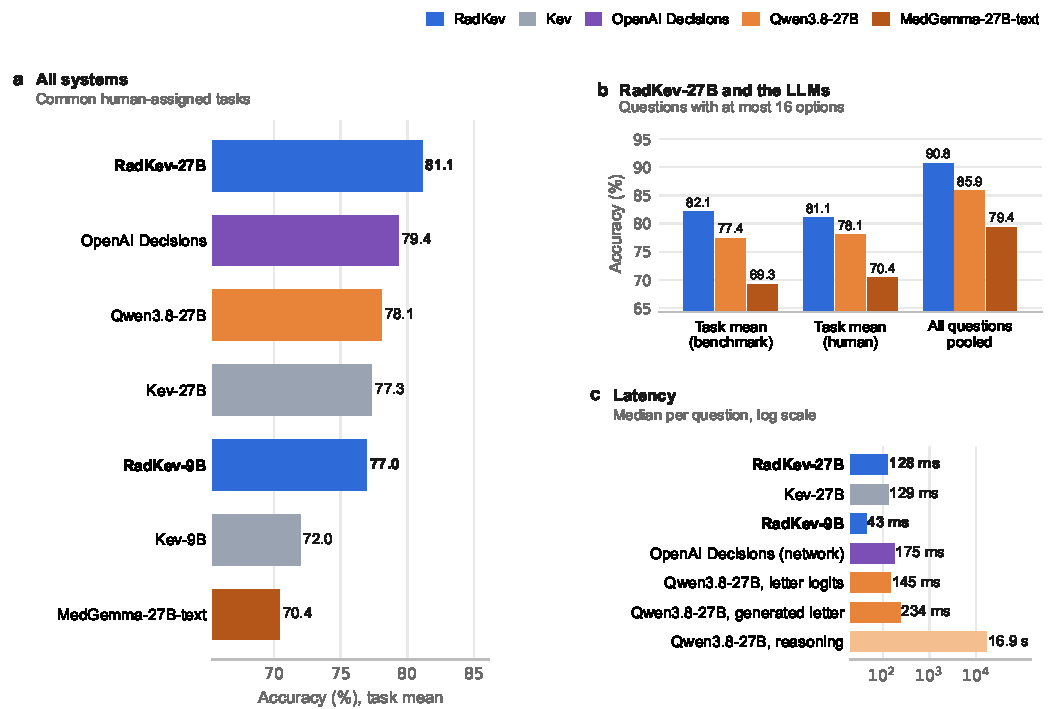
\includegraphics[width=\textwidth]{figures/v3_fig_llm.pdf}
  \caption{Decision models and language models. (a) Task-averaged accuracy of every system over the \V{r3_ncommon} human-assigned tasks that all systems answered (the LLMs were not scored on the RadCases topic question, which has \V{rc_topics} options). (b) RadKev-27B, Qwen3.8-27B and MedGemma-27B-text on the benchmark questions with at most 16 options, averaged over tasks and pooled over questions. The accuracy axes span 5 percentage points below the lowest and above the highest value. (c) Median latency per question, one request at a time on two RTX A6000 GPUs (logarithmic axis); a decision model answers all questions about a record in one pass, Qwen3.8-27B was scored from its option-letter logits, by generating the answer letter, or with reasoning, and the hosted OpenAI Decisions API was timed end to end from the institution's network, one request at a time (\V{r3_lt_od_seq_n} requests). Blue, RadKev; grey, the other decision models (Kev, light; OpenAI Decisions, dark); tan, the LLMs (MedGemma-27B-text, dark; Qwen3.8-27B with reasoning, light).}
  \label{fig:llm}
\end{figure}

On the \V{r3_ncommon} human-assigned tasks that every system answered, task-averaged accuracy was \V{r3_c_v3_27}\% for RadKev-27B, \V{r3_c_openai_dec}\% for the OpenAI Decisions API, \V{r3_c_qwen38}\% for Qwen3.8-27B, \V{r3_c_stock27}\% for Kev-27B, \V{r3_c_v3_9}\% for RadKev-9B, \V{r3_c_stock9}\% for Kev-9B and \V{r3_c_medgemma_fix}\% for MedGemma-27B-text (Figure~\ref{fig:llm}a; Supplementary Table~\ref{tab:v3_pertask}). % [C7]
On the questions with at most 16 options (\V{r3_q_ntask} tasks), RadKev-27B was \V{r3_q_tm_cmp} Qwen3.8-27B, its own backbone queried as an LLM (task mean, \V{r3_q_tm} points, 95\% CI \V{r3_q_tm_ci}; over the \V{r3_q_hntask} human-assigned tasks, \V{r3_q_htm} points, \V{r3_q_htm_ci}), and \V{r3_mg_tm_cmp} MedGemma-27B-text (\V{r3_mg_tm} points, \V{r3_mg_tm_ci}; Figure~\ref{fig:llm}b; Supplementary Table~\ref{tab:v3_pairs}). % [C4] [C5]
The differences from Qwen3.8-27B ranged by task from \V{r3_q_tmin} points (\V{r3_q_tmin_task}) to \V{r3_q_tmax} points (\V{r3_q_tmax_task}) and were positive on \V{r3_q_npos} of \V{r3_q_ntask} tasks. % [C16]
Before specialization, Qwen3.8-27B was \V{r3_qk_tm_cmp} Kev-27B (\V{r3_qk_tm} points, \V{r3_qk_tm_ci}). % [C6]
RadKev-9B was \V{r3_q9_tm_cmp} Qwen3.8-27B (\V{r3_q9_tm} points, \V{r3_q9_tm_ci}).
The hosted OpenAI Decisions API (gpt-6-luna), a general-purpose decision model, reached a benchmark task mean of \V{r3_a_openai_dec_tm}\%. RadKev-27B was \V{r3_od_tm_cmp} it (\V{r3_od_tm} points, \V{r3_od_tm_ci}; over the human-assigned tasks, \V{r3_od_htm} points, \V{r3_od_htm_ci}), with per-task differences from \V{r3_od_tmin} points (\V{r3_od_tmin_task}) to \V{r3_od_tmax} points (\V{r3_od_tmax_task}), and RadKev-9B was \V{r3_od9_tm_cmp} it (\V{r3_od9_tm} points, \V{r3_od9_tm_ci}). The API declined \V{r3_od_refusals} of the \V{r3_nq} questions, which were scored as a uniform distribution over their options. Measured end to end from the institution's network, its median latency per question was \V{r3_lt_od} ms with four requests in flight (\V{r3_lt_od_n} requests) and \V{r3_lt_od_seq} ms with one request at a time (\V{r3_lt_od_seq_n} requests), and the processing time reported by the API was \V{r3_lt_od_server} ms per request (median). % [C23]
In the post hoc analysis with reasoning enabled, on a sample of \V{r3_rs_q} benchmark questions on which every system was scored, Qwen3.8-27B reached \V{r3_rs_qwen38}\% without and \V{r3_rs_qwen38_think}\% with reasoning (\V{r3_rp_qthink} points, \V{r3_rp_qthink_ci}), and MedGemma-27B-text \V{r3_rs_medgemma_think}\% with reasoning; RadKev-27B, which does not reason, reached \V{r3_rs_v3_27}\%, a difference from Qwen3.8-27B with reasoning of \V{r3_rp_rk_qthink} points pooled over questions (\V{r3_rp_rk_qthink_ci}) and \V{r3_rp_rk_qthink_tm} points averaged over the \V{r3_rs_ntk} tasks of the sample, with the examination questions pooled into one task (\V{r3_rp_rk_qthink_tm_ci}; Supplementary Table~\ref{tab:v3_reasoning} and Supplementary Note~S4).
On \V{r3_lat_records} benchmark records timed one request at a time, the median latency per question was \V{r3_lt_rk27} ms for RadKev-27B and \V{r3_lt_rk9} ms for RadKev-9B, compared with \V{r3_lt_q} ms for Qwen3.8-27B scored from its option-letter logits, \V{r3_lt_qgen} ms when it generated the answer letter and \V{r3_lt_qthink} s with reasoning, about \V{r3_lt_ratio_think} times the latency of RadKev-27B (Figure~\ref{fig:llm}c; Supplementary Table~\ref{tab:v3_latency}). % [manual] letter-scored LLM about as fast; gains only vs generation and reasoning

\FloatBarrier
\subsection{Specialization and scale}\label{sec:res_spec}

Specialization changed the benchmark task mean by \V{r3_prim_tm} points at 27B and by \V{r3_spec9_tm} points at 9B (\V{r3_spec9_tm_ci}), and the threefold increase in size from Kev-9B to Kev-27B changed it by \V{r3_scale_tm} points (\V{r3_scale_tm_ci}; Figure~\ref{fig:spec}a); the difference between the two gains (specialization minus scale) was \V{r3_did27_tm} points at 27B (\V{r3_did27_tm_ci}) and \V{r3_did9_tm} points at 9B (\V{r3_did9_tm_ci}); the latter equals the difference between RadKev-9B and Kev-27B, so the specialized 9B model was \V{r3_r9k27_tm_cmp} the general-purpose model three times its size. % [C9]
Over the human-assigned tasks, the gain from specialization at 27B (\V{r3_prim_htm} points) was \V{r3_specscale_h} that from scale (\V{r3_scale_htm} points; difference \V{r3_did27_htm}, \V{r3_did27_htm_ci}), whereas pooled over the human-assigned questions, of which IU/Open-i report reading forms the majority, the corresponding gains were \V{r3_prim_hpool} and \V{r3_scale_hpool} points (difference \V{r3_did27_hpool}, \V{r3_did27_hpool_ci}; Figure~\ref{fig:spec}b), so the comparison of specialization with scale depends on how tasks are weighted. % [C8]
On Kev's out-of-domain transfer suite (\V{r3_transfer_n} questions), which measures general decision skill outside radiology, accuracy changed by \V{r3_tr_9} points for RadKev-9B relative to Kev-9B (\V{r3_tr_9_ci}) and by \V{r3_tr_27} points for RadKev-27B relative to Kev-27B (\V{r3_tr_27_ci}; Figure~\ref{fig:spec}c; Supplementary Table~\ref{tab:v3_transfer}).

\begin{figure}[!htb]
  \centering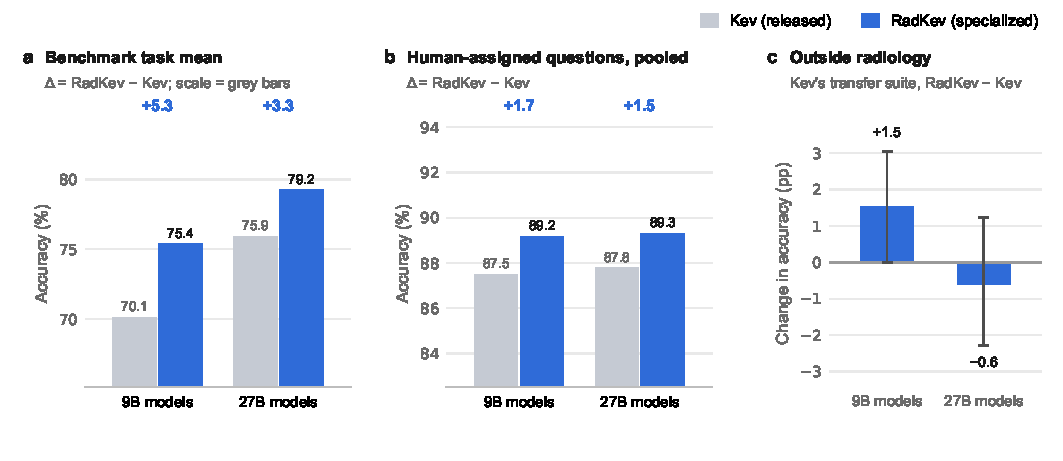
\includegraphics[width=\textwidth]{figures/v3_fig_spec.pdf}
  \caption{Specialization and scale. The released Kev models (grey) and their specialized counterparts, RadKev (blue), at 9B and 27B, as the benchmark task mean (a) and pooled over the human-assigned questions (b); the gain from specialization is the difference within each pair, and the gain from scale is the difference between the two grey bars. Each accuracy axis spans 5 percentage points below the lowest and above the highest value. (c) Change in accuracy on Kev's out-of-domain transfer suite, specialized minus released model; whiskers, 95\% confidence intervals.}
  \label{fig:spec}
\end{figure}

\FloatBarrier
\subsection{Calibration and selective prediction}\label{sec:res_calib}

On the human-assigned questions, answered in descending order of confidence, RadKev-27B could answer \V{r3_cal_v3_27_cov}\% of them with an error rate of at most 5\% among the answered questions, compared with \V{r3_cal_stock27_cov}\% for Kev-27B (\V{r3_calp_cov} points, 95\% CI \V{r3_calp_cov_ci}), \V{r3_cal_qwen38_cov}\% for Qwen3.8-27B, \V{r3_cal_medgemma_fix_cov}\% for MedGemma-27B-text and \V{r3_cal_openai_dec_cov}\% for the OpenAI Decisions API (RadKev-27B minus the API, \V{r3_od_cov_d} points, \V{r3_od_cov_ci}; Figure~\ref{fig:calib}a). % [C11]
Over all \V{r3_nq} benchmark questions, including the ReXErr questions, the corresponding coverage was \V{r3_bcov_v3_27}\% for RadKev-27B and \V{r3_bcov_stock27}\% for Kev-27B.
Its expected calibration error was \V{r3_cal_v3_27_ece}, compared with \V{r3_cal_stock27_ece} for Kev-27B, \V{r3_cal_qwen38_ece} for Qwen3.8-27B and \V{r3_cal_medgemma_fix_ece} for MedGemma-27B-text; its Brier score was \V{r3_cal_v3_27_brier} (Kev-27B, \V{r3_cal_stock27_brier}); and \V{r3_cal_v3_27_ce}\% of questions were answered incorrectly with a confidence of at least 0.9, compared with \V{r3_cal_stock27_ce}\% for Kev-27B (Figure~\ref{fig:calib}b,~c). After cross-fitted recalibration on the test split, the calibration errors of RadKev-27B and Kev-27B were \V{r3_rc_v3_27_ece} and \V{r3_rc_stock27_ece}, and their coverage at a 5\% error budget \V{r3_rc_v3_27_cov}\% and \V{r3_rc_stock27_cov}\% (Supplementary Table~\ref{tab:v3_calib}). % [C12]

\begin{figure}[!htb]
  \centering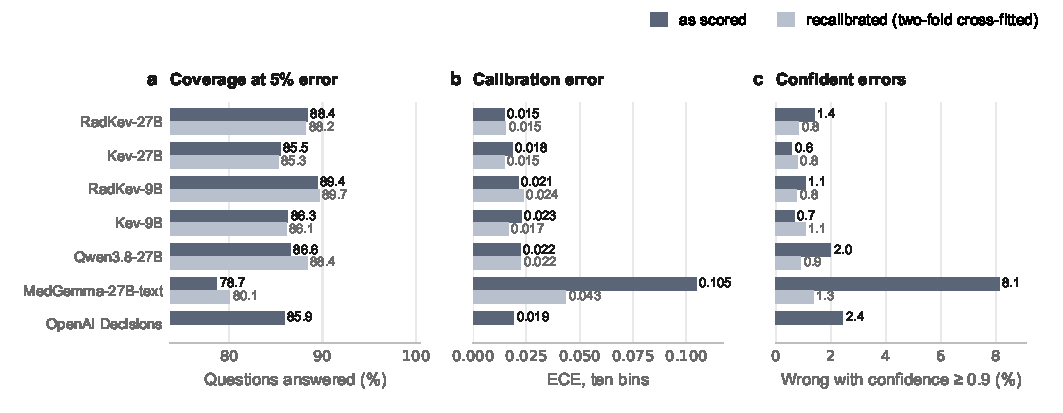
\includegraphics[width=\textwidth]{figures/v3_fig_calib.pdf}
  \caption{Calibration and selective prediction on the \V{r3_nhq} human-assigned benchmark questions. (a) Proportion of questions that can be answered, in descending order of confidence, with at most 5\% error among the answered questions. (b) Expected calibration error over ten equal-width confidence bins. (c) Questions answered incorrectly with a confidence of at least 0.9. Dark bars show the models as scored, each with its own temperature, and light bars after two-fold cross-fitted temperature recalibration on the test split, which leaves accuracy unchanged. The OpenAI Decisions API returns probabilities rounded to two decimals and is shown as scored only.}
  \label{fig:calib}
\end{figure}

\FloatBarrier
\subsection{Robustness of the gains}\label{sec:res_robust}

When the Eurorad subspecialty question was posed with the imaging findings removed, leaving the age, sex and clinical history that are available before a study is read, the accuracy of every system fell, by \V{r3_pr_minchg} to \V{r3_pr_maxchg} percentage points (\V{r3_pr_n} questions; Figure~\ref{fig:robust}a; Supplementary Table~\ref{tab:v3_preread}). % [C13]
RadKev-27B reached \V{r3_pr_v3_27_pre}\% before the read and \V{r3_pr_v3_27_full}\% with the findings; before the read, its difference from Kev-27B was \V{r3_prp_prim_pre} points (\V{r3_prp_prim_pre_ci}) and that from Qwen3.8-27B \V{r3_prp_q_pre} points (\V{r3_prp_q_pre_ci}). % [C14]
On the IU/Open-i, Eurorad and examination questions, the gain of RadKev-27B over Kev-27B was \V{r3_wd_held} points on instruction wordings withheld from training (\V{r3_wd_held_ci}; \V{r3_wd_held_n} questions) and \V{r3_wd_seen} points on wordings seen in training (\V{r3_wd_seen_ci}; \V{r3_wd_seen_n} questions), a difference of \V{r3_wd_did} points (\V{r3_wd_did_ci}); for RadKev-9B, the corresponding gains were \V{r3_wd9_held} (\V{r3_wd9_held_ci}) and \V{r3_wd9_seen} points (\V{r3_wd9_seen_ci}), a difference of \V{r3_wd9_did} points (\V{r3_wd9_did_ci}; Figure~\ref{fig:robust}b). % [C17]
In the options-only control, in which the case was removed and only the question and its answer options were shown, the accuracy of RadKev-27B on Eurorad diagnosis fell from \V{r3_bl_dx_rk27_full}\% to \V{r3_bl_dx_rk27}\%, that of Kev-27B from \V{r3_bl_dx_k27_full}\% to \V{r3_bl_dx_k27}\%, that of Qwen3.8-27B from \V{r3_bl_dx_q_full}\% to \V{r3_bl_dx_q}\% and that of MedGemma-27B-text from \V{r3_bl_dx_mg_full}\% to \V{r3_bl_dx_mg}\%, against \V{bl_chance_dx}\% expected by chance (Figure~\ref{fig:robust}c). The gain from specialization was larger without the case (\V{r3_bl_dx_gain_blind} points, \V{r3_bl_dx_gain_blind_ci}) than with it (\V{r3_bl_dx_gain_full} points, \V{r3_bl_dx_gain_full_ci}; difference \V{r3_bl_dx_did}, \V{r3_bl_dx_did_ci}), and at 9B it was \V{r3_bl_dx9_gain_blind} points without and \V{r3_bl_dx9_gain_full} points with the case. With the case available, the gain was \V{r3_bl_aw_flag} points (\V{r3_bl_aw_flag_ci}) in the \V{r3_bl_aw_flag_n} questions in which a distinctive word of the correct option occurred in the case text and \V{r3_bl_aw_none} points (\V{r3_bl_aw_none_ci}) in the \V{r3_bl_aw_none_n} in which none did, so it did not depend on words of the correct diagnosis appearing in the case. The specialized models therefore recognized the case author's final diagnosis among the differential diagnoses from the answer options themselves, and the gain on Eurorad diagnosis does not indicate improved reading of the case. % [C18]
On RSNA-RadioQA, whose incorrect options were written by LLMs, options-only accuracy was \V{r3_bl_rsna_rk27}\% for RadKev-27B, \V{r3_bl_rsna_k27}\% for Kev-27B and \V{r3_bl_rsna_q}\% for Qwen3.8-27B, against 25\% expected by chance; the gain from specialization was \V{r3_bl_rsna_gain_blind} points without the case (\V{r3_bl_rsna_gain_blind_ci}) and \V{r3_bl_rsna_gain_full} points with it (\V{r3_bl_rsna_gain_full_ci}; Figure~\ref{fig:robust}d; Supplementary Table~\ref{tab:v3_blind}).

\begin{figure}[!htb]
  \centering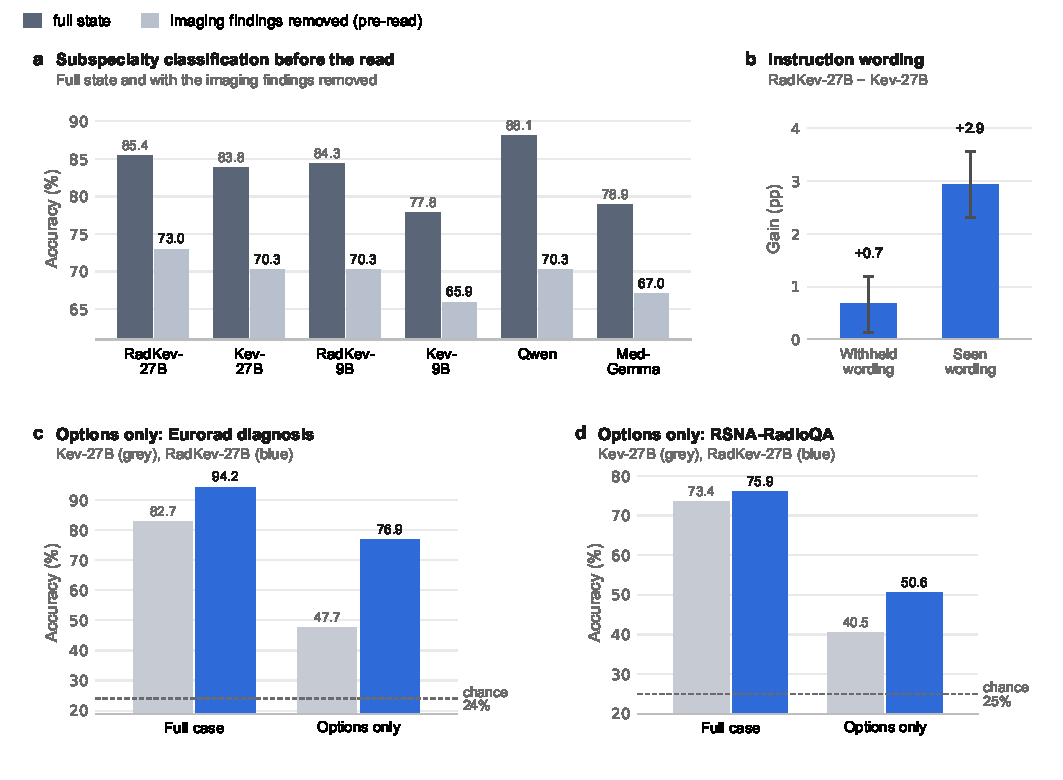
\includegraphics[width=\textwidth]{figures/v3_fig_robust.pdf}
  \caption{Robustness of the gains. (a) Eurorad subspecialty classification with the full state (dark) and with the imaging findings removed (light), as before the read; accuracies as recomputed in this analysis (Supplementary Table~\ref{tab:v3_preread}). (b) Gain of RadKev-27B over Kev-27B on instruction wordings withheld from and seen in training; whiskers, 95\% confidence intervals. (c, d) Options-only control: accuracy of Kev-27B (grey) and RadKev-27B (blue) with the full case and with only the question and its options, for Eurorad diagnosis (c) and RSNA-RadioQA (d); a model that needs the case should fall to chance (dashed lines).}
  \label{fig:robust}
\end{figure}

\FloatBarrier
\subsection{Size and composition of the answer space}\label{sec:res_answerspace}

In the answer-space analysis of \V{r3_as_n_dx} Eurorad diagnosis and \V{r3_as_n_rsna} RSNA-RadioQA questions, in which the case and the correct answer were held fixed and the other options replaced by 1 to 254 alternatives, accuracy depended more on how similar the alternatives were to the correct answer than on how many were offered (Supplementary Table~\ref{tab:v3_answer_space}). With the 16 most similar Eurorad diagnoses as options, the accuracy of RadKev-27B was \V{r3_as_rk27_dx_sim16}\%, compared with \V{r3_as_k27_dx_sim16}\% for Kev-27B, \V{r3_as_q_dx_sim16}\% for Qwen3.8-27B and \V{r3_as_mg_dx_sim16}\% for MedGemma-27B-text (Figure~\ref{fig:answerspace}); with 255 options, it was \V{r3_as_rk27_dx_rand255}\% with random and \V{r3_as_rk27_dx_sim255}\% with the most similar alternatives. On RSNA-RadioQA, with the 16 most similar alternatives, the accuracy of RadKev-27B was \V{r3_as_rk27_rsna_sim16}\%, compared with \V{r3_as_k27_rsna_sim16}\% for Kev-27B, \V{r3_as_q_rsna_sim16}\% for Qwen3.8-27B and \V{r3_as_mg_rsna_sim16}\% for MedGemma-27B-text. The LLMs were scored by generating the number of the chosen option and, with up to 16 options, also from the probabilities of single-letter option labels; the decision models score each option directly. On \V{r3_as_lat_cases} Eurorad cases with one question per request, the latency of RadKev-27B rose from \V{r3_as_lat_rk27_2} ms with two options to \V{r3_as_lat_rk27_255} ms with 255. The latency of Qwen3.8-27B rose from \V{r3_as_lat_q_2} ms with two options to \V{r3_as_lat_q_255} ms with 255 when it generated the number of its chosen option, and was \V{r3_as_lat_qletter_2} to \V{r3_as_lat_qletter_16} ms for 2 to 16 options when scored from the probabilities of the option letters. % [C21]

\begin{figure}[!htb]
  \centering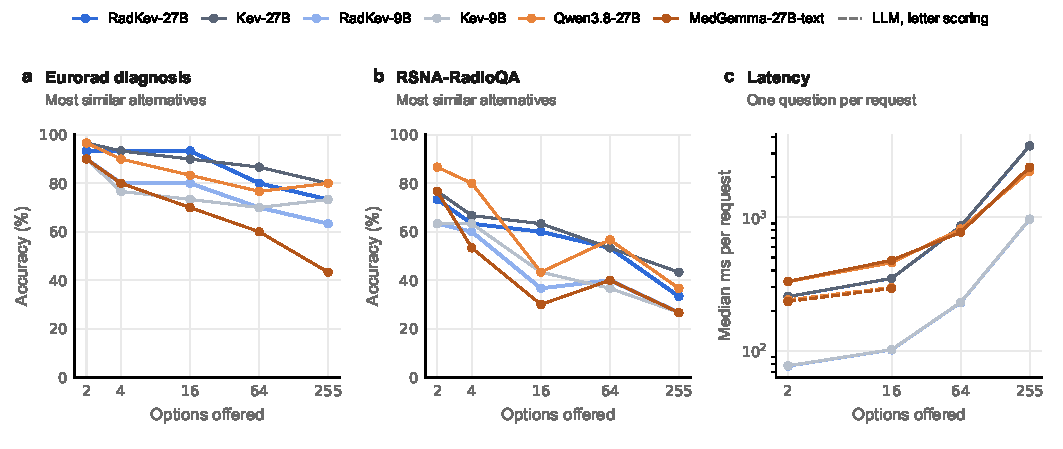
\includegraphics[width=\textwidth]{figures/v3_fig_answer_space.pdf}
  \caption{Accuracy and latency as the answer space grows (2, 4, 16, 64 and 255 options): \V{r3_as_n_dx} Eurorad diagnosis and \V{r3_as_n_rsna} RSNA-RadioQA questions with the correct answer offered together with the most similar alternatives, and median latency per request with one question per request on \V{r3_as_lat_cases} Eurorad cases, in which the lines of RadKev and Kev models of the same size coincide. The LLMs were scored by generating the number of the chosen option. Results with random and LLM-written alternatives are given in Supplementary Table~\ref{tab:v3_answer_space}; Supplementary Note~S5 describes the construction of the answer spaces.}
  \label{fig:answerspace}
\end{figure}

\FloatBarrier
\subsection{External test set}\label{sec:res_external}

On the \V{r3_rg_n} RadGraph-XL status questions from CT and MRI reports of another institution, accuracy was \V{r3_rg_v3_27}\% for RadKev-27B and \V{r3_rg_stock27}\% for Kev-27B (\V{r3_rg_d} points, 95\% CI \V{r3_rg_d_ci}), \V{r3_rg_qwen38}\% for Qwen3.8-27B (\V{r3_rg_dq} points, \V{r3_rg_dq_ci}) and \V{r3_rg_medgemma_fix}\% for MedGemma-27B-text; at 9B, the difference from specialization was \V{r3_rg_d9} points (\V{r3_rg_d9_ci}; Supplementary Table~\ref{tab:supp_external}). The decision models frequently classified hedged findings, which RadGraph-XL annotates as uncertain, as present: such findings formed \V{r3_rgu_share}\% of the questions and were answered correctly by RadKev-27B in \V{r3_rgu_v3_27}\%, by Kev-27B in \V{r3_rgu_stock27}\% and by Qwen3.8-27B in \V{r3_rgu_qwen38}\% of cases, and they accounted for \V{r3_rgu_qwin_unc} of the \V{r3_rgu_qwin} questions that only Qwen3.8-27B answered correctly. Uncertain findings formed \V{r3_rgu_train_share}\% of the status answers in the training data.
